% Name: Dependency graph
% Description: Course prerequisites as a directed acyclic graph, laid out in layers from left to right.
% Tags: DAG, dependencies, topological order, prerequisites

\usetikzlibrary{arrows.meta}

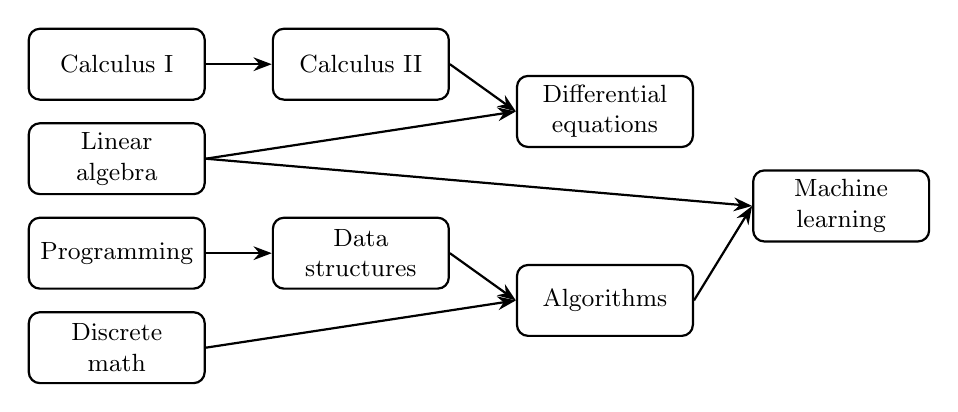
\begin{tikzpicture}[
  >={Stealth},
  course/.style={draw, thick, rounded corners, text width=20mm, align=center, minimum height=9mm, font=\small},
]
  \node[course] (calc1) at (0,1.8) {Calculus I};
  \node[course] (linalg) at (0,0.6) {Linear algebra};
  \node[course] (prog) at (0,-0.6) {Programming};
  \node[course] (disc) at (0,-1.8) {Discrete math};
  \node[course] (calc2) at (3.1,1.8) {Calculus II};
  \node[course] (ds) at (3.1,-0.6) {Data structures};
  \node[course] (ode) at (6.2,1.2) {Differential equations};
  \node[course] (algo) at (6.2,-1.2) {Algorithms};
  \node[course] (ml) at (9.2,0) {Machine learning};

  \foreach \a/\b in {calc1/calc2, calc2/ode, linalg/ode, prog/ds, ds/algo, disc/algo, linalg/ml, algo/ml}
    \draw[->, thick] (\a.east) -- (\b.west);
\end{tikzpicture}
